\section{Struttura}
\subsection{Informazioni Generali}
Per la modellazione dei database di Utenti e Prodotti è stata utilizzata la struttura dati
\textbf{list} messa a disposizione della libreria STL.
Il database degli utenti è una semplice lista che contiene puntatori agli utenti, che possono essere di tipo differente, mentre il database dei tavoli è una lista di puntatori a tavoli, che possono essere di tipo differente. Ogni tavolo può contenere un puntatore ad una lista di consumazioni.
La gestione del garbage è affidata alle singole funzioni di eliminazione.

\subsection{Pattern MVC}
Durante la realizzazione del progetto si è cercato di seguire il più possibile l'architettura del pattern Model-View-Controller, separando l'implementazione grafica da quella logica. 
I primi controlli nell'inserimento dati vengono affidati alla View, mentre quelli derivati da vincoli logici al controller.
Ogni classe è dotata di opportuni metodi "get" e/o "set".

\subsection{Implementazione GUI}
Per quanto riguarda l'implementazione dell'interfaccia grafica, poiché non significativamente complessa, la codifica è stata effettuata "a mano", senza utilizzare quindi tool del Framework di Qt.
Al fine di evitare ripetizione eccessiva di codice alcune finestre adattano diversamente il loro layout in base alla necessità.
Le varie schermate utilizzano
un oggetto \textbf{QGridLayout} per disporre in maniera ordinata gli
oggetti al loro interno.
La gestione della distruzione degli oggetti della GUI di ogni view, viene affidata alla view stessa, poiché ogni oggetto viene aggiunto al Layout della view stessa.

\subsection{Gerarchia Utenti}
\begin{figure}[htbp]
\centering
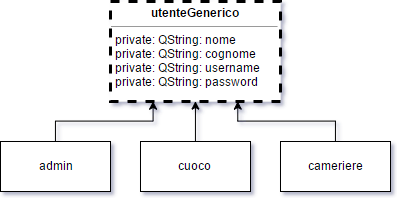
\includegraphics[scale=0.7]{res/sections/immagini/utenti.png}
\caption{Gerarchia utenti}
\end{figure}

\subsubsection{Base astratta utente generico}
Rappresenta l'astrazione del concetto utente, oltre agli attributi riportati nella figura precedente presenta i seguenti metodi:

\textbullet \verb|virtual QString getTipo() const=0|:
restituisce una QString contenente il tipo dell'utente, utilizzato al fine di non usare eccessivamente dynamic-cast ove non strettamente necessario;

\textbullet \verb|virtual bool canDoTavolo()const=0|: 
restituisce un booleano a seconda che l'utente da cui viene invocato abbia permessi di modifica, aggiunta e/o rimozione sui tavoli; 

\textbullet \verb|virtual bool canDoConsumazioni()const=0|:
restituisce un booleano a seconda che l'utente da cui viene invocato abbia permessi di modifica, aggiunta e/o rimozione sulle consumazioni;

\textbullet \verb|virtual bool canDoGestione()const=0|:
restituisce un booleano a seconda che l'utente da cui viene invocato abbia permessi di modifica, aggiunta e/o rimozione sugli utenti;

\textbullet \verb|virtual void saveUtente(QXmlStreamWriter& xmlWriter)=0|:
metodo virtuale puro che si occupa di procede al salvataggio dei dati utenti nel modo corretto, in relazione a come implementato per ogni sottoclasse;

\textbullet \verb|virtual void loadUtente(QXmlStreamReader& xmlReader)=0|:
metodo virtuale puro che si occupa di procede alla lettura dei dati utenti nel modo corretto, in relazione a come implementato per ogni sottoclasse.

I dati comuni a tutti gli utenti vengono caricati con i \\
metodi \verb|void loadBaseUtente(QXmlStreamReader& xmlReader)| \\
e scritti nel file con  \verb|void saveBaseUtente(QXmlStreamWriter& xmlWriter)|.

Le classi \textit{admin}, \textit{cameriere}, \textit{cuoco} si occupano di implementare i metodi virtuali della base, conferendo ad ogni utente diversi permessi.

Nel dettaglio:
\begin{centering}
	\arrayrulecolor{black}
		\begin{longtable}{|>{\centering\arraybackslash}m{2cm}|m{9cm}|}
\hline
\textbf{Ruolo}  & \textbf{Funzionalità} \\
\hline
admin  & 
\textbullet ricerca di tavoli, consumazioni e utenti\newline
\textbullet gestione(aggiunta, modifica e rimozione) tavoli, consumazioni e utenti\newline
\textbullet gestione dei propri dati utente \\ \hline

cameriere  &
\textbullet ricerca di tavoli, consumazioni e utenti\newline
\textbullet gestione(aggiunta, modifica e rimozione)consumazioni\newline
\textbullet gestione dei propri dati utente \\ \hline

cuoco  & 
\textbullet ricerca di tavoli, consumazioni e utenti\newline
\textbullet gestione dei propri dati utente \\ \hline

\caption{Riepilogo funzionalità}
		 \end{longtable}
		 \end{centering}

\subsection{Gerarchia Tavoli}
\begin{figure}[!h]
\centering
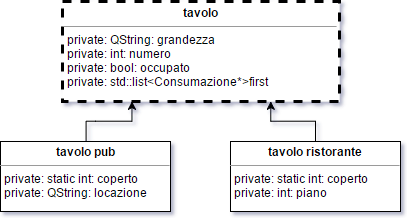
\includegraphics[scale=0.7]{res/sections/immagini/tavoli.png}
\caption{Gerarchia tavoli}
\end{figure}
\subsubsection{Base astratta tavolo}
Rappresenta l'astrazione del concetto di tavolo, oltre agli attributi riportati nella figura precedente presenta i seguenti metodi:\\
\textbullet \verb|virtual int getPosti() const=0|:
restituisce un intero che rappresenta i posti disponibili in un tavolo a seconda della grandezza dello stesso;
\\
\textbullet \verb|virtual double getCoperto() const =0|:
restituisce un double rappresentante il prezzo del coperto per il tavolo;
\\
\textbullet \verb|virtual QString getTipo()const=0|:
restituisce una QString contenente il tipo del tavolo, utilizzato al fine di non usare eccessivamente dynamic-cast ove non strettamente necessario;
\\
\textbullet \verb|virtual void saveTavolo(QXmlStreamWriter & w)=0|:
metodo virtuale puro che si occupa di procede al salvataggio dei dati del tavolo nel modo corretto, in relazione a come implementato per ogni sottoclasse;
\\
\textbullet \verb|virtual void loadTavolo(QXmlStreamReader & r)=0|:
metodo virtuale puro che si occupa di procede alla lettura dei dati utenti nel modo corretto, in relazione a come implementato per ogni sottoclasse.

I dati comuni a tutti i tavoli vengono caricati con i \\
metodi \verb|void loadBaseTavolo(QXmlStreamReader& r))| \\
e scritti nel file con  \verb|void saveBaseTavolo(QXmlStreamWriter& xmlWriter)|.

Non vengono salvate su file le consumazioni aggiunte ai tavoli.
    
\subsubsection{Classe concreta tavolo pub}
Ogni tavolo pub ha un campo dati statico constante che rappresenta il coperto.
Questa classe modella la rappresentazione di un tavolo nel ristorante con una locazione che può essere esterna o interna. 
\subsubsection{Classe concreta tavolo ristorante}
Ogni tavolo ristorante ha un campo dati statico constante che rappresenta il coperto.
Questa classe modella la rappresentazione di un tavolo nel ristorante che si trova ad un piano indicato dall'utente.
\subsection{Classe concreta consumazioni}
\begin{figure}[htbp]
\centering
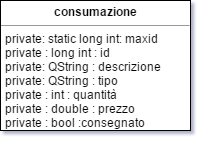
\includegraphics[scale=0.7]{res/sections/immagini/consumazione.png}
\caption{Classe consumazione}
\end{figure}

Modella gli oggetti che sono contenuti nei tavoli. Ogni consumazione ha un id univoco.
Le consumazioni non vengono salvate nel file .xml.
Alla terminazione del programma i dati a loro associati andranno persi.
